\begin{figure}[htbp]
\centering
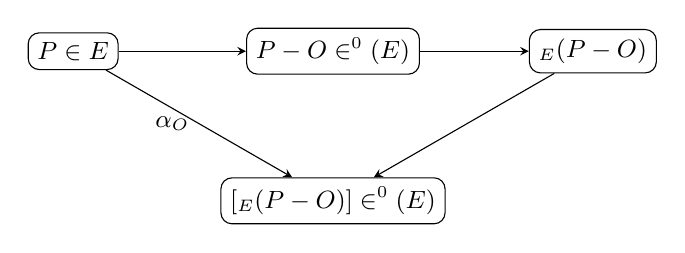
\begin{tikzpicture}[>=stealth,every node/.style={font=\small}]
\node[draw,rounded corners] (p) at (-3.3,0.9) {$P\in E$};
\node[draw,rounded corners] (d) at (0,0.9) {$P-O\in\Div^0(E)$};
\node[draw,rounded corners] (l) at (3.3,0.9) {$\OO_E(P-O)$};
\node[draw,rounded corners] (c) at (0,-1.0) {$[\OO_E(P-O)]\in\Pic^0(E)$};
\draw[->] (p) -- (d);
\draw[->] (d) -- (l);
\draw[->] (l) -- (c);
\draw[->] (p) -- node[left] {$\alpha_O$} (c);
\end{tikzpicture}
\caption{For a smooth plane cubic, the Abel--Picard map identifies points with degree-zero line-bundle classes.}
\label{fig:vi43-abel-picard}
\end{figure}
